\documentclass[final]{beamer}
\usetheme{ISR}
\usepackage[orientation=landscape,size=a1,scale=1.4,debug]{beamerposter}
\usepackage[absolute,overlay]{textpos}
\setlength{\TPHorizModule}{1cm}
\setlength{\TPVertModule}{1cm}

\title{A Formally Verified SCUBA Dive Computer Based on Commodity Sensors}
\author{Viren Bajaj  \and Karim Elmaroufi \and Nathan Fulton \and Andre Platzer\\
    vbajaj@andrew.cmu.edu}

\footer{Viren Bajaj $\cdot$ vbajaj@andrew.cmu.edu $\cdot$ https://github.com/nrfulton/scuba-release}
\date{}



%%%%%%%%%%%%%%%%%%%%%%%%%%%%%%%%%%%%%%%%%%%%%%%%%%%%%%%%%%%%%%%%5

\usepackage{afterpage}
\usepackage{listings}
\usepackage{mathpartir}
\usepackage{amsmath}
\usepackage{amssymb} 
\usepackage{dL}
\usepackage{multicol}
\usepackage{bm}

%%%%%%%%%%%%%%%%%%%%%%%%%%%%%%%%%%%%%%%%%%%%%%%%%%%%%%%%%%%%%%%%5


\usepackage{amsthm}
\newtheorem{thm}{Theorem}                                                       
\newtheorem{cor}[thm]{Corollary}                                                
\newtheorem{lem}[thm]{Lemma}                                                    
\newtheorem{prop}[thm]{Proposition}                                             
\newtheorem{ax}[thm]{Axiom}                                                     
\theoremstyle{definition}                                                       
\newtheorem{defn}[thm]{Definition}                                              
\newtheorem{exam}[thm]{Example}                                                 
\newtheorem{rem}[thm]{Remark}                                                   

%%%%%%%%%%%%%%%%%%%%%%%%%%%%%%%%%%%%%%%%%%%%%%%%%%%%%%%%%%%%%%%%%

\begin{document}
\begin{frame}[fragile]

%%%%%%%%%%%%%%%%%%%%%%%%%%%%%%%%%%%%%%%%%%%%%%%%%%%%%%%%%%%%%%%%%
% The QR code -- if you do not want this, simply comment out 
% all three lines.
%%%%%%%%%%%%%%%%%%%%%%%%%%%%%%%%%%%%%%%%%%%%%%%%%%%%%%%%%%%%%%%%%

\begin{textblock}{10}(1,1)

\includegraphics[height=3cm]{images/scuba_qr.png}
\end{textblock}

%%%%%%%%%%%%%%%%%%%%%%%%%%%%%%%%%%%%%%%%%%%%%%%%%%%%%%%%%%%%%%%%%
% Text sections
%%%%%%%%%%%%%%%%%%%%%%%%%%%%%%%%%%%%%%%%%%%%%%%%%%%%%%%%%%%%%%%%%

\begin{textblock}{27}(2,5.5)

\begin{block}{Abstract}
We present a model of a novel, formally verified \textbf{low-cost dive computer} which calculates oxygen consumption using the diver's heart rate in order to increase the time underwater and reduce the risk of decompression sickness. To monitor air supply, current cutting edge dive computers utilize a pressure gauge fixed on the tank that connects to a wrist watch through a wireless transmitter. Not only is this method very expensive, but it also adds a single point failure into a safety-critical system. 

Our \textbf{novel approach toward safe diving} uses a commodity heart rate sensor and a mathematical model relating oxygen consumption and heart rate. Using these primitives, we calculate the volume of air remaining in the diver's tank. The safety of our SCUBA safety monitor is established using the highly trustworthy KeYmaera X theorem prover for Hybrid Systems.
%Our resulting model could be used as a stand-alone, \textbf{low-cost} device to monitor oxygen consumption in recreational settings. Our system is also appropriate as a fallback mechanism even when sophisticated equipment is available.
\end{block}
\begin{block}{Overview}
Ensuring safe SCUBA diving requires reasoning about how the physical world will evolve in between two sensor measurements. We rely on \textbf{commodity heart-rate and depth sensors} together with a \textbf{mathematical model} relating heart rate to oxygen consumption.
\hfill \break

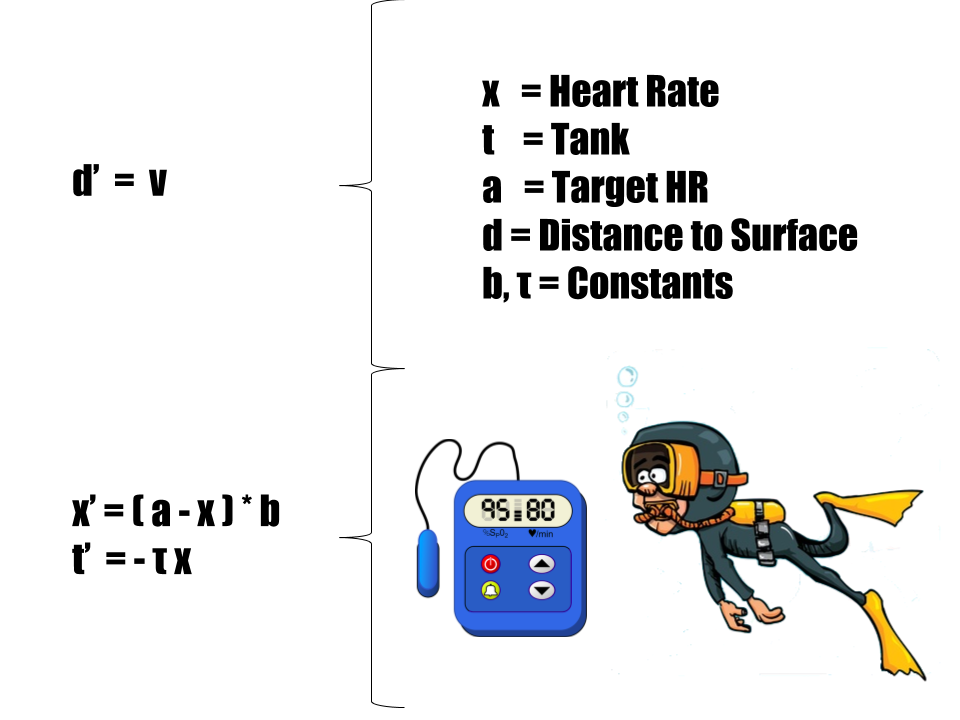
\includegraphics[width = 26cm,scale=.75]{images/SCUBA.png}\\
Based on this model, we derive a control policy that allows the diver a range of movements while still ensuring that the diver can return to the surface without running out of oxygen. Using KeYmaera X, we developed the first formally verified SCUBA dive computer.
\end{block}
\end{textblock}



%%%%%%%%%%%%%%%%%%%%%%%%%%%%%%%%%%%%%%%%%%%%%%%%%%%%%%%%%%%%%%%%%
% The Carnegie Mellon University logo
%%%%%%%%%%%%%%%%%%%%%%%%%%%%%%%%%%%%%%%%%%%%%%%%%%%%%%%%%%%%%%%%%

\begin{textblock}{23}(2.0,53)

\includegraphics[height=4.5cm,width=25.365cm]{images/SCS_Unitmark_187_K_CMYK.png}
\end{textblock}

%%%%%%%%%%%%%%%%%%%%%%%%%%%%%%%%%%%%%%%%%%%%%%%%%%%%%%%%%%%%%%%%%
% Main Sections 
%%%%%%%%%%%%%%%%%%%%%%%%%%%%%%%%%%%%%%%%%%%%%%%%%%%%%%%%%%%%%%%%%

\begin{textblock}{51}(31,5.5)

\begin{block}{Model}
\begin{multicols}{2}
\begin{align*}
\underbrace{t \ge 0 \land \dotsm \vphantom{\dibox{}}}_{\text{precondition}} & 
\limply 
\dibox{\prepeat{ \{ ctrl;
\{ \underbrace{\textit{ascend} \cup \textit{stay} \cup \textit{descend}}_{\text{diver's behavioral model}} \}; plant 
\}
}}\underbrace{\textit{tank} \ge 0}_{\text{postcondition}}
\label{eq:carmodel}
\end{align*}

\begin{align*}
\bm{ctrl} &\equiv \{\texttt{NOP} \cup \humod{t_{worst}}{t}\} \\\\
\bm{ascend} &\equiv \{\humod{a}{*};\humod{v}{v_{asc}} \} \\\\
\bm{stay} &\equiv \{?t_{worst} \ge \tau hr_{max} \epsilon
        + \tau hr_{max}  \frac{-d}{v_{asc}};\\
        &\hspace{1.5cm}\humod{a}{*};\humod{v}{0}\} \\\\
\bm{descend} &\equiv \{?t_{worst} \ge \tau*hr_{max} * \epsilon
        + \tau hr_{max}  \frac{-d - v_{desc}\epsilon}{v_{asc}};\\
        &\hspace{1.5cm}\humod{a}{*}; \humod{v}{0}\} \\\\
\bm{plant} &\equiv  \humod{c}{0}; \\
          &\hspace{1.1cm}\{x' = b(a-x),\\
          &\ \hspace{1.1cm}t' = -\tau x,\\
          &\ \hspace{1.1cm}d' = v,\\
          &\ \hspace{1.1cm}c' = 1 \\
          &\ \hspace{1.1cm}\text{\& } d \ge 0 ~\land~c \le \epsilon\} \\
          &\hspace{1.1cm}\{\humod{t_{worst}}{t_{worst} - \tau hr_{max} c}\} 
\end{align*}

\columnbreak

Our hybrid system program model is comprised of a controller, a behavioural model of the diver, a model of the physical world (\textit{plant}), and a safety specification.
\hfill \break

\begin{itemize}
    \item The \textbf{controller} models the diver's ability to occasionally update the controller's approximation of the the tank volume ($t_{worst}$) to the actual value of the tank ($t$). The non-deterministic choice $\cup$ means that the system is safe even if the diver never updates the controller's over-approximation of the available oxygen.
    \hfill \break 
    \item The \textbf{diver's behavioral model} splits the diver's kinematic decision space into three cases based on his vertical velocity, each of which has a different safety condition. 
    \hfill \break 
    \item The \textbf{plant} relates heart rate, oxygen consumption, and the diver's vertical movement. 
    \hfill \break 
    \item The \textbf{safety specification} is comprised of the initial conditions for which the system is safe and the post condition which ensures that the tank is never empty. 
    
\end{itemize}
\hfill \break 
Our \textbf{computer-checked proof} of safety for this system makes use of advanced proof techniques, including \emph{differential ghosts} to establish the invariant set $HR_{min} \le x \le HR_{max}$ and differential invariants to propagate safety constraints from the controller through the continuous dynamics.



% \begin{itemize}
%     \item The first equation describes the dynamics of the heart rate (\textit{x}) in response to exercise. The diver's level of exertion determines a steady state heart rate (\textit{a}).
%     \item  The second equation describes the rate of oxygen consumption as a function of heart rate.
%     \item The third and fourth equations describe the depth and time dynamics.
%     \item After each control step, the controller approximates the oxygen consumed over the previous time step, assuming the diver's heart rate is always at its maximum value. Because this is a worst-case assumption, the controller safely over-approximates the amount of oxygen consumed ($t_{worst}$).
% \end{itemize}
  



\end{multicols}



\end{block}

\begin{block}{Simulations}
\begin{multicols}{3}
Subject: male, age 33\\
Height: 1.33m\\ 
Weight: 82 kg \\\columnbreak
$V0_{2}^{max}$: 49.7 ml $min^{-1}$ $kg^{-1}$ \\
$HR_{max}$: 185 \\
$HR_{min}$: 40\\\columnbreak
b = 0.1968\\
$\tau$=0.483 ml $s^{-1}$
\end{multicols}

\vspace{5mm}
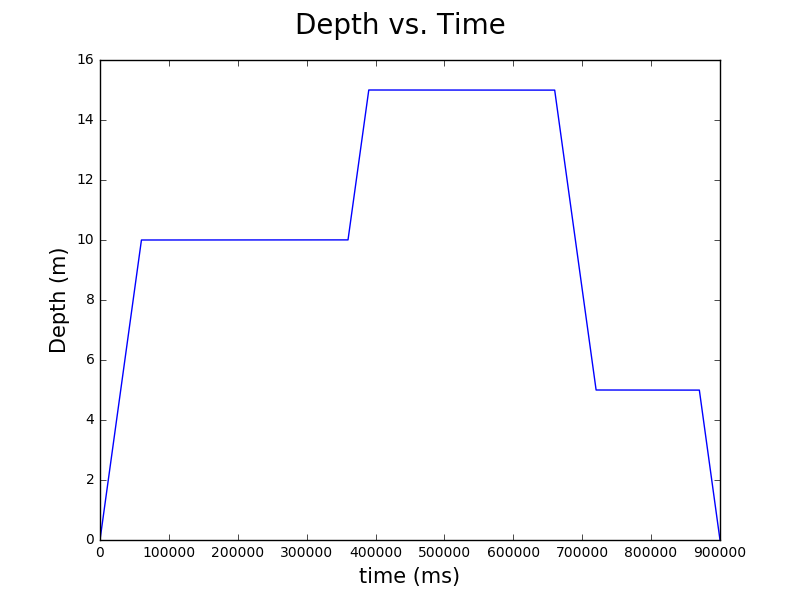
\includegraphics[scale=.8]{images/depthDynamics_15min.png}\hspace{5mm}
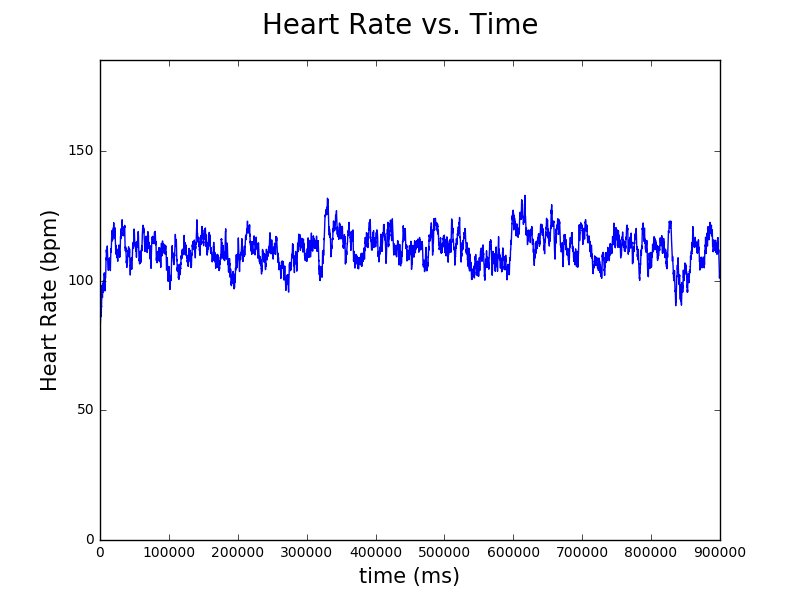
\includegraphics[scale=.8]{images/hrDynamics_15min.png}\hspace{5mm}
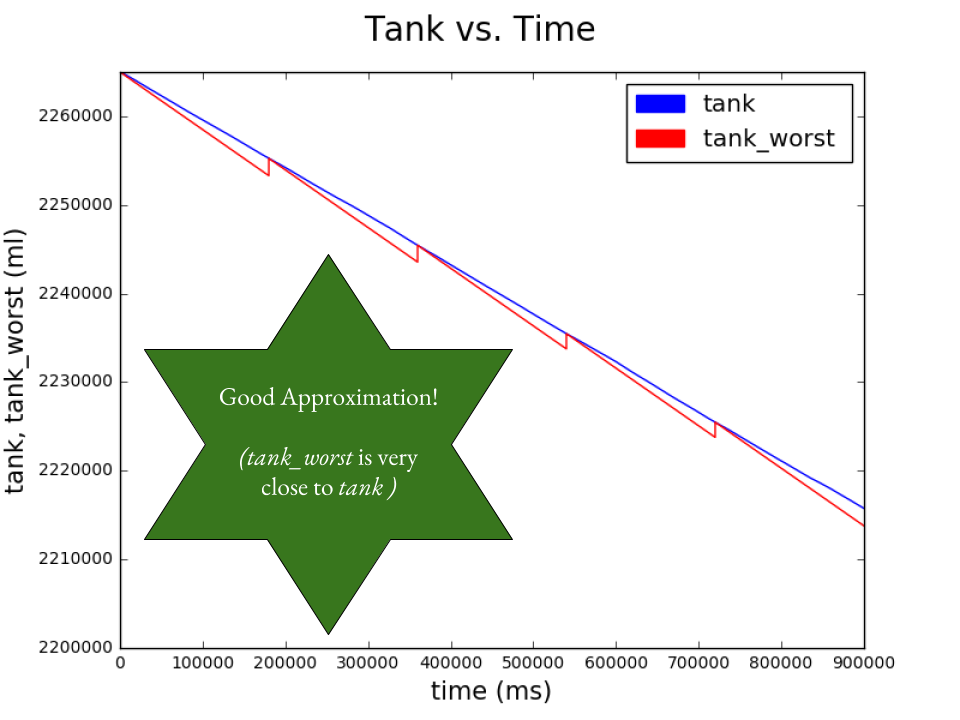
\includegraphics[scale=.48]{images/_tankDynamics(1).png}

\end{block}

%%%%%%%%%%%%%%%%%%%%%%%%%%%%%%%%%%%%%%%%%%%%%%%%%%%%%%%%%%%%%%%%%
% The ISR Logo 
%%%%%%%%%%%%%%%%%%%%%%%%%%%%%%%%%%%%%%%%%%%%%%%%%%%%%%%%%%%%%%%%%



\end{textblock}

\end{frame}
\end{document}
